\chapter{ANALISIS DAN PERANCANGAN SISTEM} \label{chap:analisis-perancangan-sistem}
\tab Pada bab ini dijelaskan mengenai analisis dan perancangan sistem perangkat lunak yang akan dibangun, meliputi struktur data, algoritme, dan arsitektur aplikasi. 

\section{Daftar Notasi}
\tab Daftar notasi yang digunakan dalam bab ini dideskripsikan pada Tabel \ref{tab:daftar-notasi-1} dan \ref{tab:daftar-notasi-2}.

\begin{longtable}{| p{3cm} | p{6cm} |} 
	\caption{Daftar notasi (bagian 2) \label{tab:daftar-notasi-2}}\\
	\hline
	\textbf{Notasi} & \textbf{Deskripsi}\\ \hline
	\endfirsthead
	\hline
	\textbf{Notasi} & \textbf{Deskripsi}\\ \hline
	\endhead
	$[t_i:t_e]$ & Interval waktu \\ \hline
	$E$ & Himpunan \textit{event} \\ \hline
	$e$ & Sebuah \textit{event} dalam $E$, $e \in E$ \\ \hline
	$p_{i}$ & Data produk masuk \\ \hline
	$p_{o}$ & Data produk keluar \\ \hline
	$c_{i}$ & Data pelanggan masuk \\ \hline
	$c_{o}$ & Data pelanggan keluar \\ \hline
	$PA$ & Himpunan data produk yang sedang aktif \\ \hline	
	$CA$ & Himpunan data pelanggan yang sedang aktif \\ \hline
	$diff$ & Selisih nilai \\ \hline
	$Pr_t(c, p|PA)$ & Probabilitas produk $p \in PA$ dibeli oleh pelanggan $c \in CA$ pada waktu $t$ \\ \hline
	$E_t(CA, p|PA)$ & Kontribusi pasar $p$ pada waktu $t$ \\ \hline
	$E_{[t_i:t_e]}(CA, p|PA)$ & Kontribusi pasar $p$ dalam interval waktu $[t_i:t_e]$\\ \hline
	$k-MPPTI$ & \textit{k-Most Promising Products in Time Intervals} \\ \hline
	$PB$ & \textit{Pandora Box} \\ \hline
\end{longtable}

\section{Analisis Sistem}
\tab Analisis sistem dijelaskan dalam empat bagian, yakni analisis permasalahan, deskripsi umum sistem, fungsi sistem, dan analisis kebutuhan fungsional.

\subsection{Analisis Permasalahan}
\tab Permalasahan yang ingin diselesaikan pada Tugas Akhir ini adalah bagaimana menjawab kueri \textit{k-Most Promising Products} berbasis interval waktu (k-MPPTI). Interval waktu, dinotasikan dengan $[t_i:t_e ](t_i \leq t_e)$, digunakan untuk menentukan rentang waktu pencarian. Permasalahan ini tidak dapat langsung diselesaikan menggunakan metode dan algoritme yang sudah ada \cite{kmpp}. Sehingga, diperlukan pendekatan lain yang akan dijelaskan pada bagian perancangan sistem.

\subsection{Deskripsi Umum Sistem}
\tab Secara umum, sistem yang akan dibangun adalah sebuah sistem berbasis web yang dapat membantu pengguna untuk memilih \textit{k}-produk yang paling menjanjikan. Dikatakan "menjanjikan" jika produk tersebut memiliki kontribusi pasar yang besar.

Sistem ini memiliki dua proses utama, yaitu (1) \textit{data precomputing} untuk menghitung kontribusi pasar masing-masing produk dan (2) proses utama (selanjutnya akan disebut dengan \textit{query processing}) untuk memproses dan menampilkan hasil kueri pencarian yang dimasukkan oleh pengguna.

Sistem ini dibangun menggunakan arsitektur \textit{client}-\textit{server}. Aplikasi \textit{client} didesain berbasis web dengan memanfaatkan Flask \textit{microframework}, HTML, CSS, dan JavaScript. Selain itu, Flask juga digunakan sebagai \textit{web server}. 

\subsection{Fungsi Sistem}
\tab Sistem yang akan dibangun memiliki beberapa fungsi utama sebagai berikut:
\begin{enumerate}
	\item Dapat menerima masukan data berupa file dari pengguna
	\item Dapat menampilkan informasi dan pratinjau data yang dimasukkan oleh pengguna
	\item Dapat menampilkan visualisasi data
	\item Dapat melakukan proses \textit{data precomputing} menggunakan algoritme yang dipilih oleh pengguna
	\item Dapat menerima masukan kueri pencarian 
	\item Dapat memproses kueri pencarian
	\item Dapat menampilkan hasil kueri
\end{enumerate}

\subsection{Analisis Kebutuhan Fungsional}
\tab Sistem yang dibuat harus mampu memenuhi beberapa fungsi utama yang telah dijelaskan pada sub-bagian sebelumnya. Fungsi-fungsi ini merupakan hasil dari analisis kebutuhan fungsional dari pengguna yang dijelaskan pada Tabel \ref{tab:kebutuhan-fungsional}.

\begin{table}[H]
	\centering
	\begin{tabular}{ | p{2cm} | p{7cm} | }
		\hline
		\textbf{Kode} & \textbf{Deskripsi Kebutuhan} \\ \hline \hline
		F-001 & Mengunggah data \\ \hline
		F-002 & Melihat informasi dan pratinjau data \\ \hline
		F-003 & Melihat visualisasi data  \\ \hline
		F-004 & Memilih algoritme yang digunakan untuk \textit{data precomputing}\\ \hline
		F-005 & Memasukkan kueri pencarian \\ \hline
		F-006 & Melihat hasil kueri \\ \hline
	\end{tabular} \caption{Kebutuhan fungsional}
	\label{tab:kebutuhan-fungsional}
\end{table}

Penjelasan rinci dari masing-masing kebutuhan fungsional pada tabel \ref{tab:kebutuhan-fungsional} dijelaskan sebagai berikut:
\begin{enumerate}
	\item Mengunggah data\\
	Pengguna dapat mengunggah data produk dan preferensi pelanggan dalam bentuk file berekstensi csv.
	\item Melihat informasi dan pratinjau data \\
	Pengguna dapat melihat informasi dan pratinjau dari data yang dimasukkan berupa tabel sebanyak dua puluh baris. Informasi yang ditampilkan antara lain jumlah baris, jumlah kolom, dan nama kolom.
	\item Melihat visualisasi data \\
	Pengguna juga dapat melihat visualisasi dari data yang dimasukkan berupa lini masa sederhana.
	\item Memilih algoritme yang digunakan untuk \textit{data precomputing} \\
	Pengguna dapat memilih algoritme yang akan digunakan untuk \textit{data precomputing}, yaitu algoritme k-MPPTI dan \textit{Brute Force}.
	\item Memasukkan kueri pencarian \\
	Pengguna dapat memasukkan kueri pencarian berupa jumlah produk ($k$) dan interval waktu.
	\item Melihat hasil kueri \\
	Pengguna dapat melihat hasil kueri pencarian berupa $k$-produk dengan jumlah kontribusi pasar terbesar beserta skor kontribusi pasar-nya. 
\end{enumerate}

\section{Perancangan Sistem}
\tab Perancangan sistem akan dibagi menjadi empat bagian, yakni struktur data, algoritme, dan arsitektur aplikasi. 

\subsection{Struktur Data}
\tab Struktur data adalah suatu cara untuk menyimpan, menyusun, mengelompokkan, dan merepresentasikan suatu data. Ada tiga struktur data utama yang digunakan dalam komputasi k-MPPTI, yaitu \textit{Data Storage}, \textit{Event Queue}, dan \textit{Pandora Box}.

\subsubsection{\textit{Data Storage}}
\tab \textit{Data Storage} adalah sebuah struktur data \textit{dictionary} yang digunakan untuk menyimpan data produk dan pelanggan. Struktur data \textit{dictionary} lebih efisien untuk pencarian data karena menggunakan konsep \textit{key-value pairs}, berbeda dengan struktur data \textit{list} atau \textit{array} yang menggunakan indeks untuk mengakses nilai suatu data.

Struktur data \textit{dictionary} yang digunakan berbentuk \textit{nested dictionary} yang terdiri dari dua \textit{key} utama, yaitu '$product$' yang menyimpan data produk dan '$customer$' yang menyimpan data pelanggan. Struktur \textit{nested key} masing-masing data dijelaskan pada Gambar \ref{fig:sd1} dan \ref{fig:sd2} dan deskripsinya dijelaskan pada Tabel \ref{tab:desc-key}.

\begin{figure}[H]
	\centering
	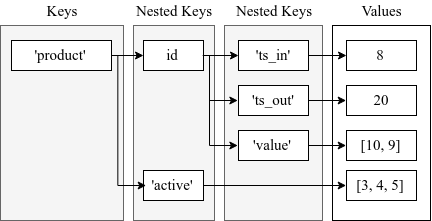
\includegraphics[width=7cm]{assets/img/bab3/sd1.png}
	\caption{Struktur data \textit{dictionary} produk}
	\label{fig:sd1}
\end{figure}

\begin{figure}[H]
	\centering
	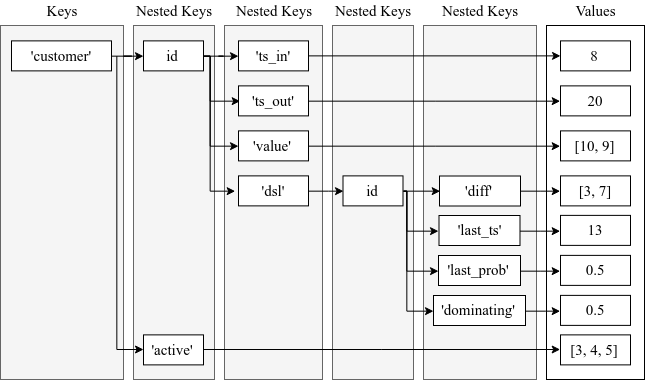
\includegraphics[width=9cm]{assets/img/bab3/sd2.png}
	\caption{Struktur data \textit{dictionary} pelanggan}
	\label{fig:sd2}
\end{figure}

\begin{longtable}{| p{2.5cm} | p{6.5cm} |}
	\caption{\textit{Key} dari \textit{DataStorage} \label{tab:desc-key}}\\
	\hline
	\textbf{\textit{Key}} & \textbf{Deskripsi} \\ \hline 
	\endfirsthead
	\hline
	\textbf{\textit{Key}} & \textbf{Deskripsi} \\ \hline 
	\endhead
	$'product'$ & Menyimpan data produk \\ \hline
	$'customer'$ & Menyimpan data pelanggan \\ \hline
	$id$ & ID data produk atau pelanggan dijadikan sebagai \textit{key} \\ \hline
	$'active'$ & Menyimpan ID data produk atau pelanggan yang sedang aktif dalam bentuk \textit{array} \\ \hline
	$'ts\_in'$ & Menyimpan \textit{timestamp} atau waktu masuk \\ \hline
	$'ts\_out'$ & Menyimpan \textit{timestamp} atau waktu keluar \\ \hline
	$'value'$ & Menyimpan nilai data produk atau pelanggan pada semua dimensi dalam bentuk \textit{array}\\ \hline
	$'dsl'$ & Menyimpan hasil \textit{dynamic skyline} dalam bentuk \textit{dictionary} dengan $id$ produk sebagai \textit{key}\\ \hline
	$'diff'$ & Menyimpan selisih antara nilai data produk dan pelanggan pada masing-masing dimensi \\ \hline
	$'last\_ts'$ & Menyimpan \textit{timestamp} terakhir saat diperbarui ke \textit{Pandora Box}\\ \hline
	$'last\_prob'$ & Menyimpan probabilitas terakhir saat diperbarui ke \textit{Pandora Box}\\ \hline
	$'dominating'$ & Menyimpan ID produk lain yang pernah didominasi\\ \hline
\end{longtable}

\subsubsection{\textit{Event Queue}}
\tab \textit{Event Queue} adalah sebuah struktur data \textit{queue} dengan prinsip FIFO (\textit{First In First Out}) yang berfungsi untuk menyimpan semua titik terjadinya perubahan di dalam himpunan data, yaitu jika ada data yang masuk atau keluar. Titik-titik ini disebut dengan \textit{event}. 

\pagebreak
Ada empat jenis \textit{event} yang terjadi: (1) data produk masuk, (2) data produk keluar, (3) data pelanggan masuk, dan (4) data pelanggan keluar. Masing-masing \textit{event} memiliki empat jenis informasi yang disimpan, yaitu \textit{timestamp}, \textit{role} (produk atau pelanggan), ID data, dan aksi (masuk atau keluar).

\begin{table}[H]
	\centering
	\begin{tabular}{|p{2cm}|p{6cm}|}
		\hline
		\textbf{Atribut} & \textbf{Deskripsi} \\ \hline \hline
		$timestamp$ & Waktu terjadinya \textit{event} \\ \hline
		$role$ & Produk $= 0$, Pelanggan $= 1$) \\ \hline
		$dataId$ & ID data\\ \hline
		$action$ & Jenis aksi yang dilakukan (masuk $= 0$, keluar $= 1$) \\ \hline
	\end{tabular} 
	\caption{Atribut dari \textit{EventQueue}}
	\label{tab:attr-event-queue}
\end{table}

\subsubsection{\textit{Pandora Box}}
\tab \textit{Pandora Box} adalah sebuah struktur data \textit{array} dua dimensi yang terdiri dari sumbu $x$ (\textit{time series}) dan sumbu $y$ (produk). Struktur data ini digunakan untuk menyimpan skor kontribusi pasar produk pada setiap waktu. Menggunakan contoh \textit{dataset} pada Tabel \ref{tab:dataset2}, maka model \textit{Pandora Box} yang terbentuk adalah seperti pada Gambar \ref{fig:pbox}.  

\begin{figure}[h]
	\centering
	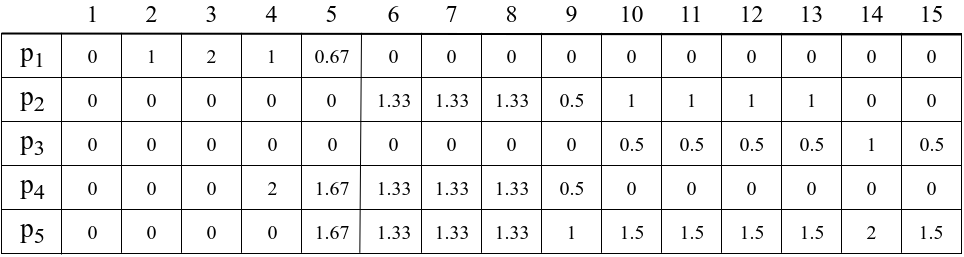
\includegraphics[width=10cm]{assets/img/bab3/pbox.png}
	\caption{Contoh \textit{Pandora Box} dari \textit{dataset} \ref{tab:dataset2}}
	\label{fig:pbox}
\end{figure}

\subsection{Algoritme Utama}
\tab Sebagaimana yang telah dijelaskan sebelumnya bahwa algoritme k-MPPTI terdiri dari dua tahap pemrosesan, yaitu \textit{data precomputing} dan \textit{query processing}. Secara garis besar, alur kerja sistem secara umum disajikan dalam bentuk diagram alir yang dapat dilihat pada Gambar \ref{fig:diagram-alur1}.

Tahap \textit{data precomputing} bertujuan untuk menghitung skor kontribusi pasar masing-masing produk berdasarkan preferensi pelanggan. Diawali dengan pembentukan \textit{Event Queue} untuk mencatat semua \textit{event} yang terjadi selama pemrosesan data. Kemudian, memproses \textit{event-event} tersebut menggunakan algoritme pemrosesan berdasarkan jenis \textit{event}-nya. Terakhir adalah mengekspor \textit{Pandora Box} untuk digunakan sebagai masukan pada tahap \textit{query processing}.

Tahap kedua adalah \textit{query processing} yang bertujuan untuk memproses kueri pencarian yang dimasukkan oleh pengguna berupa jumlah produk ($k$) dan interval waktu pencarian. Diawali dengan mencari produk sejumlah $k$ yang memiliki total skor kontribusi pasar terbesar selama interval waktu pencarian, kemudian mengembalikan hasil kueri pencarian berupa $k$-produk yang paling menjanjikan kepada pengguna.

Untuk memudahkan interaksi antara pengguna dan sistem, dibuatlah aplikasi berbasis web yang memudahkan pengguna memasukkan data produk dan pelanggan, melihat pratinjau dan visualisasi data, memasukkan kueri pencarian, serta melihat hasil kueri pencarian.

\begin{figure}[H]
	\centering
	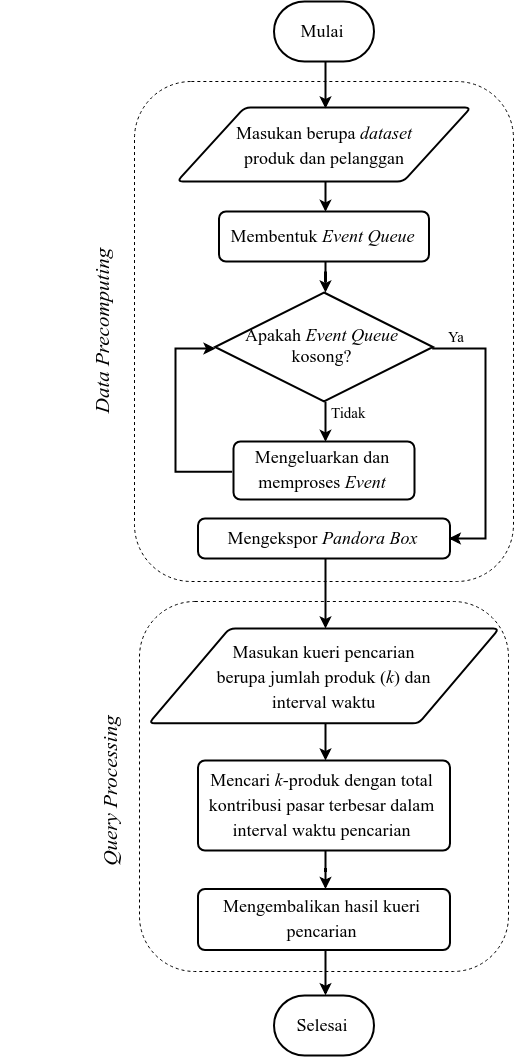
\includegraphics[width=10.5
	cm]{assets/img/bab3/flowchart.png}
	\caption{Diagram alir algoritme k-MPPTI}
	\label{fig:diagram-alur1}
\end{figure}

\subsubsection{\textit{Data Precomputing}}
\tab \textit{Data precomputing} adalah sebuah proses yang dapat menunjang performa algoritme \textit{query processing} supaya dapat bekerja lebih efektif dan efisien, yaitu dengan menghitung kontribusi pasar masing-masing produk berdasarkan preferensi pelanggan dan mengakumulasinya dalam \textit{Pandora Box}. 

Proses \textit{data precomputing} diawali dengan mencatat semua \textit{event} ke dalam \textit{Event Queue}, kemudian setiap \textit{event} diproses secara berurutan menggunakan algoritme pemrosesan berdasarkan jenis \textit{event}-nya, dan diakhiri dengan mengekspor \textit{Pandora Box} yang nantinya akan digunakan sebagai masukan pada tahap \textit{query processing}. 

Tidak adanya proses \textit{data precomputing} menyebabkan pengulangan komputasi data setiap kali seseorang memasukkan kueri pencarian. Karena data yang digunakan adalah \textit{historical data}, yaitu data yang dikumpulkan dari kejadian yang telah lalu, maka komputasi data cukup dilakukan satu kali saja di awal (\textit{precomputing}). Berbeda halnya jika data yang digunakan adalah \textit{streaming data} yang nilainya terus berubah dalam periode waktu tertentu.

Menggunakan \textit{dataset} pada Tabel \ref{tab:dataset2}, data multidimensi dengan serial waktu diilustrasikan sebagai lini masa. Lini masa atau alur waktu adalah suatu representasi kronologis urutan peristiwa atau kejadian (\textit{event}) yang dibuat menurut era, abad, tahun, bulan, minggu, atau hari. Untuk pemodelan ini, waktu direpresentasikan sebagai bilangan bulat positif dan kejadian (\textit{event}) direpresentasikan sebagai titik-titik yang dinotasikan dengan $e \in E$. 
\begin{figure}[H]
	\centering
	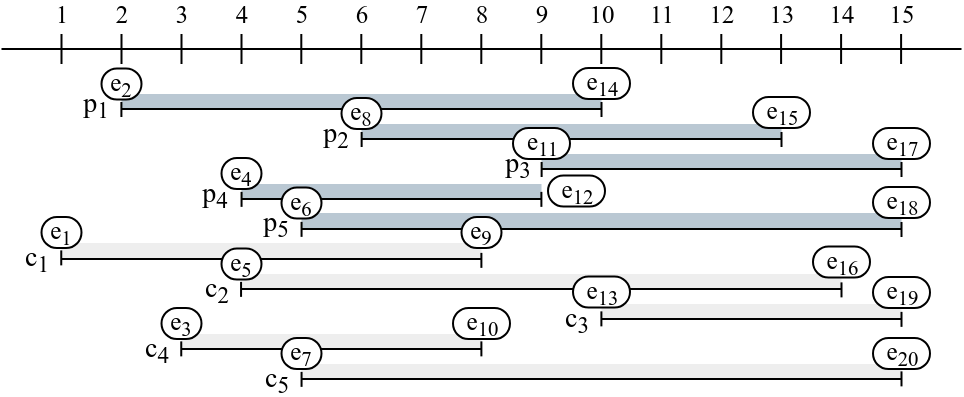
\includegraphics[width=10cm]{assets/img/bab3/timeline-event.png}
	\caption{\textit{Event} dalam lini masa data produk dan pelanggan}
	\label{fig:timeline-event}
\end{figure}

Setiap \textit{event} dicatat dan dimasukkan ke dalam \textit{Event Queue}, kemudian diproses satu persatu secara berurutan menggunakan algoritme pemrosesan berdasarkan jenis \textit{event}-nya. Contoh \textit{Event Queue} yang terbentuk dari \textit{dataset} pada Tabel \ref{tab:dataset2} ditunjukkan pada Tabel \ref{tab:event-queue}.

\begin{small}
	\begin{longtable}{|c|c|c|c|}
		\caption{\textit{EventQueue} \label{tab:event-queue}}\\
		\hline
		\multicolumn{1}{|c|}{\textbf{ID \textit{Event}}} & \multicolumn{1}{c|}{\textbf{\textit{Timestamp}}} & \multicolumn{1}{c}{\textbf{ID Data}} & \multicolumn{1}{|c|}{\textbf{Aksi}} \\ \hline 
		\endfirsthead
		\hline
		\multicolumn{1}{|c|}{\textbf{ID \textit{Event}}} & \multicolumn{1}{c|}{\textbf{\textit{Timestamp}}} & \multicolumn{1}{c}{\textbf{ID Data}} & \multicolumn{1}{|c|}{\textbf{Aksi}} \\ \hline
		\endhead
		$e_1$ & 1 & $c_1$ & Masuk \\ \hline
		$e_2$ & 2 & $p_1$ & Masuk \\ \hline
		$e_3$ & 3 & $c_4$ & Masuk \\ \hline
		$e_4$ & 4 & $p_4$ & Masuk \\ \hline
		$e_5$ & 4 & $c_2$ & Masuk \\ \hline
		$e_6$ & 5 & $p_5$ & Masuk \\ \hline
		$e_7$ & 5 & $c_5$ & Masuk \\ \hline
		$e_8$ & 6 & $p_2$ & Masuk \\ \hline
		$e_9$ & 8 & $c_1$ & Keluar \\ \hline
		$e_{10}$ & 8 & $c_4$ & Keluar \\ \hline
		$e_{11}$ & 9 & $p_3$ & Masuk \\ \hline
		$e_{12}$ & 9 & $p_4$ & Keluar \\ \hline
		$e_{13}$ & 10 & $c_3$ & Masuk \\ \hline
		$e_{14}$ & 10 & $p_1$ & Keluar \\ \hline
		$e_{15}$ & 13 & $p_2$ & Keluar \\ \hline
		$e_{16}$ & 14 & $c_2$ & Keluar \\ \hline
		$e_{17}$ & 15 & $p_3$ & Keluar \\ \hline
		$e_{18}$ & 15 & $p_5$ & Keluar \\ \hline
		$e_{19}$ & 15 & $c_3$ & Keluar \\ \hline
		$e_{20}$ & 15 & $c_5$ & Keluar \\ \hline
	\end{longtable}
\end{small}

Ada empat jenis algoritme pemrosesan berdasarkan jenis \textit{event}-nya, yaitu: (1) \textit{Product Insertion}, (2) \textit{Product Deletion}, (3) \textit{Customer Insertion}, dan (4) \textit{Customer Deletion}. Masing-masing proses itu membutuhkan dua jenis komputasi \textit{skyline}, yaitu \textit{dynamic skyline} dan \textit{reverse skyline}, sebagai metode perhitungan probabilitas dan kontribusi pasar \cite{kmpp}. 

\myparagraph{\textit{Product Insertion}}

\textit{Product insertion} adalah proses yang dijalankan ketika ada data produk yang masuk, dinotasikan dengan $p_{i}$. Adanya produk baru yang masuk memungkinkan hasil \textit{dynamic skyline} berubah sehingga komputasi harus dijalankan kembali.
 
Secara garis besar, langkah-langkah pemrosesan \textit{product insertion} adalah (1) menambahkan produk $p_{i}$ ke dalam daftar produk aktif $PA$, (2) menghitung $RSL(p_{i})$. (3) menghitung $DSL(c)$ untuk setiap $c \in RSL(p_{i})$, (4) menghitung probabilitas masing-masing produk $p \in DSL(c)$, dan (5) memperbarui \textit{Pandora Box}. Algoritme pemrosesan \textit{product insertion} disajikan dalam bentuk diagram alir pada Gambar \ref{fig:flowchart-pi}.

\begin{figure}[H]
	\centering
	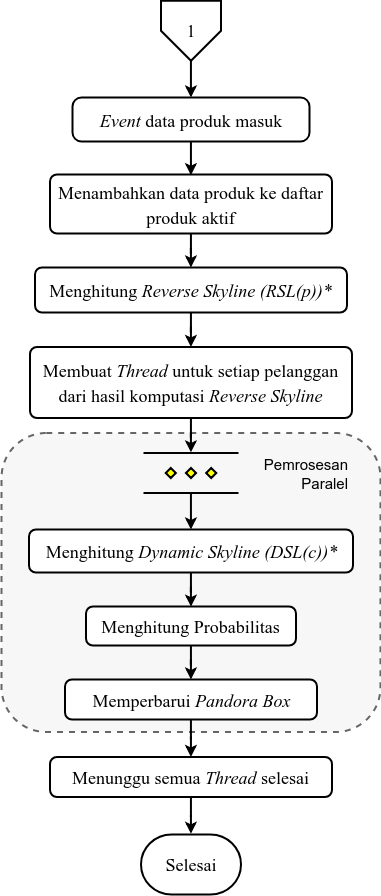
\includegraphics[width=6.5cm]{assets/img/bab3/flowchart-pi.png}
	\caption{Diagram alir proses \textit{product insertion}}
	\label{fig:flowchart-pi}
\end{figure}

\begin{figure}[H]
	\centering
	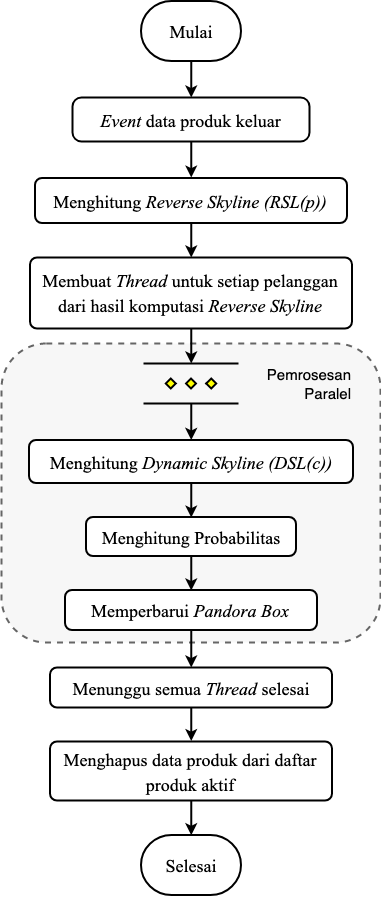
\includegraphics[width=6.5cm]{assets/img/bab3/flowchart-po.png}
	\caption{Diagram alir proses \textit{product deletion}}
	\label{fig:flowchart-po}
\end{figure}

\myparagraph{\textit{Product Deletion}}

\textit{Product deletion} adalah proses yang dijalankan ketika ada data produk yang keluar, dinotasikan dengan $p_{o}$. Adanya produk yang keluar memungkinkan hasil \textit{dynamic skyline} berubah, sehingga komputasi harus dijalankan kembali. 

Secara garis besar, langkah-langkah pemrosesan \textit{product deletion} adalah (1) memperbarui \textit{Pandora Box} untuk mengisi indeks $PB$ sebelumnya jika ada yang kosong, (2) menghitung $RSL(p_{o})$, (3) menghitung $DSL(c)$ untuk setiap $c \in RSL(p_{o})$ yang dimaksudkan untuk mencari produk-produk yang pernah didominasi (\textit{child}), (4) menghitung probabilitas masing-masing produk $p \in DSL(c)$, dan (5) menghapus produk $p_{o}$ dari daftar produk aktif $PA$. Algoritme pemrosesan \textit{product deletion} disajikan dalam bentuk diagram alir pada Gambar \ref{fig:flowchart-po}.

\myparagraph{\textit{Customer Insertion}}

\textit{Customer insertion} adalah proses yang dijalankan ketika ada data pelanggan yang masuk, dinotasikan dengan $c_{i}$. Secara garis besar, langkah-langkah pemrosesan \textit{customer insertion} adalah (1) menambahkan pelanggan $c_{i}$ ke dalam daftar pelanggan aktif $CA$, (2) menghitung \textit{initial} $DSL(c_{i})$ untuk mendapatkan hasil \textit{dynamic skyline} awal, (3) menghitung probabilitas masing-masing produk $p \in DSL(c)$, dan (4) memperbarui \textit{Pandora Box}. Algoritme pemrosesan \textit{customer insertion} disajikan dalam bentuk diagram alir pada Gambar \ref{fig:flowchart-ci}.

\myparagraph{\textit{Customer Deletion}}

\textit{Customer deletion} adalah proses yang dijalankan ketika ada data pelanggan yang keluar, dinotasikan dengan $c_{o}$. Secara garis besar, langkah-langkah pemrosesan \textit{customer deletion} adalah (1) memperbarui \textit{Pandora Box} untuk mengisi indeks $PB$ sebelumnya jika ada yang kosong dan (2) menghapus pelanggan $c$ dari daftar pelanggan aktif $CA$. Algoritme pemrosesan \textit{customer deletion} disajikan dalam bentuk diagram alir pada Gambar \ref{fig:flowchart-co}. 

\begin{figure}[H]
	\centering
	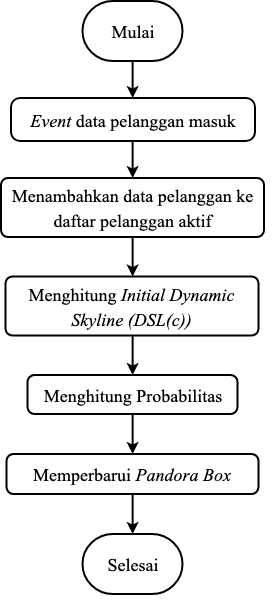
\includegraphics[width=5cm]{assets/img/bab3/flowchart-ci.png}
	\caption{Diagram alir proses \textit{customer insertion}}
	\label{fig:flowchart-ci}
\end{figure}

\begin{figure}[H]
	\centering
	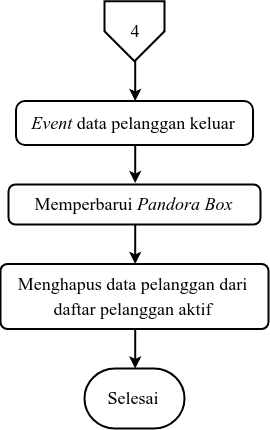
\includegraphics[width=5cm]{assets/img/bab3/flowchart-co.png}
	\caption{Diagram alir proses \textit{customer deletion}}
	\label{fig:flowchart-co}
\end{figure}

\myparagraph{\textit{Dynamic Skyline}}

Komputasi \textit{dynamic skyline} digunakan untuk mencari produk terbaik dari sudut pandang pelanggan \cite{kmpp}. Secara umum, proses komputasi \textit{dynamic skyline} diawali dengan perhitungan selisih absolut dari nilai masing-masing dimensi antara pelanggan dan produk, dinotasikan dengan: $diff^i = |c^i - p^i|$.

Selanjutnya, mengecek dominansi dinamis antar produk dengan membandingkan selisih absolut-nya. Sebagai contoh, ada dua produk yang akan dibandingkan, dinotasikan dengan $p_1$ sebagai subjek dan $p_2$ sebagai objek pembanding. Berdasarkan syarat dominansi dinamis (Persamaan \ref{eq:syarat-dominansi-dinamis}), $p_1$ dikatakan mendominasi $p_2$ jika dan hanya jika:
\begin{equation}\label{eq:komputasi-dsl}
\begin{split}
\text{(a)} \tab diff_1^i \leq diff_2^i, \forall i \in [1, ..., d] \\
\text{(b)} \tab diff_1^i < diff_2^i, \exists i \in [1, ..., d]
\end{split}
\end{equation}
Pengecekan dominansi dinamis dilakukan secara iteratif hingga dipastikan suatu $p_1$ tidak didominasi oleh $p_2$ lain sama sekali. Jika $p_1$ tidak pernah didominasi, maka $p_1$ menjadi hasil $DSL(c)$.

\begin{figure}[H]
	\centering
	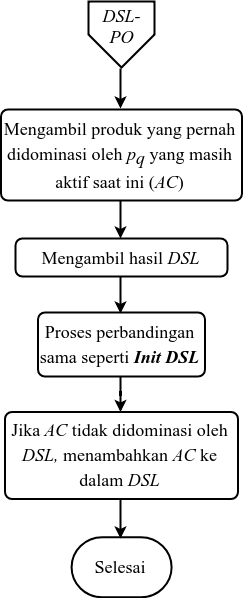
\includegraphics[width=4.5cm]{assets/img/bab3/flowchart-dsl-pd.png}
	\caption{Diagram alir komputasi \textit{dynamic skyline - product deletion}}
	\label{fig:flowchart-dsl-pd}
\end{figure}

\begin{figure}[H]
	\centering
	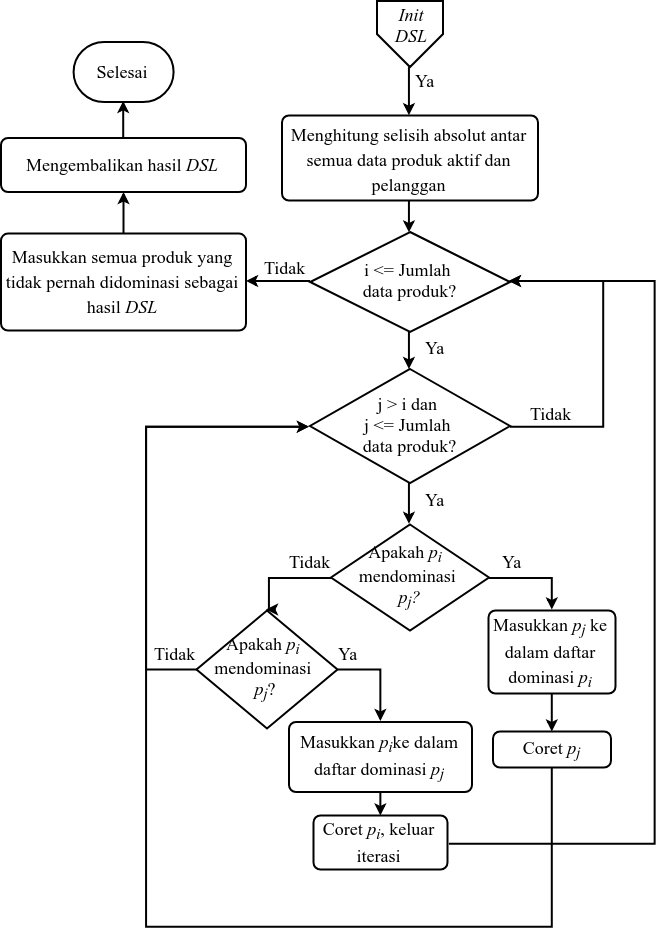
\includegraphics[width=10cm]{assets/img/bab3/flowchart-dsl-init.png}
	\caption{Diagram alir komputasi \textit{initial dynamic skyline}}
	\label{fig:flowchart-dsl-init}
\end{figure}

\begin{figure}[H]
	\centering
	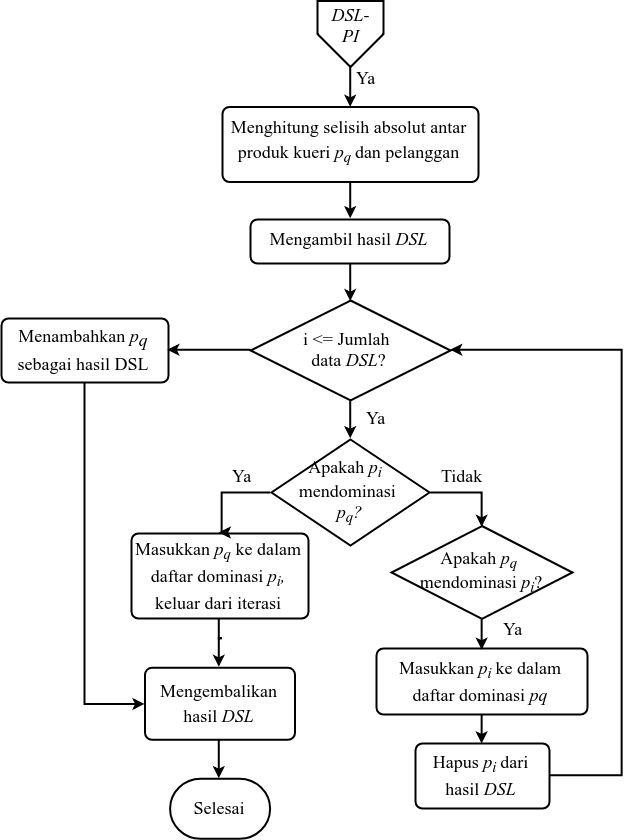
\includegraphics[width=10cm]{assets/img/bab3/flowchart-dsl-pi.png}
	\caption{Diagram alir komputasi \textit{dynamic skyline - product  insertion}}
	\label{fig:flowchart-dsl-pi}
\end{figure}

\pagebreak
Algoritme komputasi $DSL$ dalam k-MPPTI dibagi menjadi 3 jenis, yaitu: (1) \textit{InitDSL} yang dijalankan jika ada data pelanggan yang masuk, diilustrasikan dalam bentuk diagram alir pada Gambar \ref{fig:flowchart-dsl-init}; (2) \textit{DSL-PI} yang dijalankan jika ada data produk yang masuk, diilustrasikan dalam bentuk diagram alir pada Gambar \ref{fig:flowchart-dsl-pi}; (3) \textit{DSL-PD} yang dijalankan jika ada data produk yang keluar, diilustrasikan dalam bentuk diagram alir pada Gambar \ref{fig:flowchart-dsl-pd}.

\myparagraph{Komputasi \textit{Reverse Skyline}}

Komputasi \textit{reverse skyline} digunakan untuk mencari pelanggan potensial dari sudut pandang produsen \cite{kmpp}. Komputasi \textit{reverse skyline} diawali dengan menentukan \textit{orthant} dari produk, dinotasikan dengan $O$. Dalam geometri, \textit{orthant} adalah analog dalam ruang data \textit{d}-dimensi atau biasa dikenal sebagai kuadran dalam bidang dua dimensi. Setiap produk $p$ memiliki $2^d$ \textit{orthant} pada data $d-$dimensi. 

\textit{Orthant} ditandai menggunakan bilangan biner. Sebagai contoh, terdapat empat \textit{orthant} pada bidang dua dimensi, yaitu $O_{00}$, $O_{01}$, $O_{10}$, dan $O_{11}$, dan delapan \textit{orthant} pada bidang tiga dimensi, yaitu $O_{000}$ hingga $O_{111}$. Penggunaan bilangan biner bertujuan untuk menandai batas wilayah sebuah \textit{orthant}. Misalnya, \textit{orthant} $O_{010}$ dari produk $p_1$ memiliki wilayah dengan batas-batas sebagai berikut: sumbu $x [0:pos_x(p_1)]$, sumbu $y [pos_y(p_1):max_y]$, dan sumbu $z [0:pos_z(p_1)]$.

Langkah selanjutnya adalah menghitung \textit{midpoint} atau titik tengah antara produk kueri dan produk $p \in P$ menggunakan Persamaan \ref{eq:midpoint}. Kemudian, menentukan \textit{midpoint skyline} pada setiap \textit{orthant} $MSL(o)$. Komputasi diakhiri dengan menentukan \textit{reverse skyline} dengan mencari semua pelanggan $c \in C$ yang tidak didominasi oleh \textit{midpoint skyline} $m \in M$ berdasarkan produk $p_1$, $c \nprec_{p_1} m$. Untuk lebih jelasnya, komputasi \textit{reverse skyline} diilustrasikan dalam bentuk diagram alir pada Gambar \ref{fig:flowchart-rsl}.

\myparagraph{Pengecekan Dominasi}

Pengecekan dominasi antar data digunakan dalam setiap komputasi \textit{dynamic skyline} dan \textit{reverse skyline}. Sebagaimana syarat dominansi dinamis yang telah dijelaskan pada Persamaan \ref{eq:syarat-dominansi-dinamis} dan \ref{eq:komputasi-dsl}, dominasi antar data ditentukan dengan membandingkan selisih absolut data dengan titik kueri secara iteratif sejumlah dimensi data. Supaya lebih jelas, proses pengecekan dominasi diilustrasikan dalam bentuk diagram alir pada Gambar \ref{fig:flowchart-cek-dom}.

\myparagraph{Perhitungan Probabilitas}

Setelah mendapatkan hasil \textit{dynamic skyline} dan \textit{reverse skyline}, probabilitas masing-masing produk $p \in PA$ dipilih oleh pelanggan $c \in CA$ dihitung menggunakan Persamaan \ref{eq:prob-ti}.
\begin{equation}\label{eq:prob-ti}
Pr_t(c, p|PA) = \left\{
\begin{array}{ll}
\frac{1}{|DSL(c)|} & \text{if } p \in DSL(c)\\
0 & \text{otherwise}\\
\end{array}
\right.
\end{equation}

\myparagraph{Perhitungan Kontribusi Pasar}

Kontribusi pasar produk $p$, dinotasikan dengan $E(C, p|P)$, diperoleh dengan mengakumulasikan probabilitas produk dari setiap pelanggan $c \in RSL(p)$ sebagaimana Persamaan \ref{eq:mc}, kemudian skornya disimpan dalam \textit{Pandora Box}.
\begin{equation}\label{eq:mc}
E_t(CA, p|PA) = \sum_{\forall c \in RSL(p)} Pr_t(c, p|P)
\end{equation}
Perhitungan probabilitas dan kontribusi pasar dilakukan setiap akhir pemrosesan \textit{event}.

\begin{figure}[H]
	\centering
	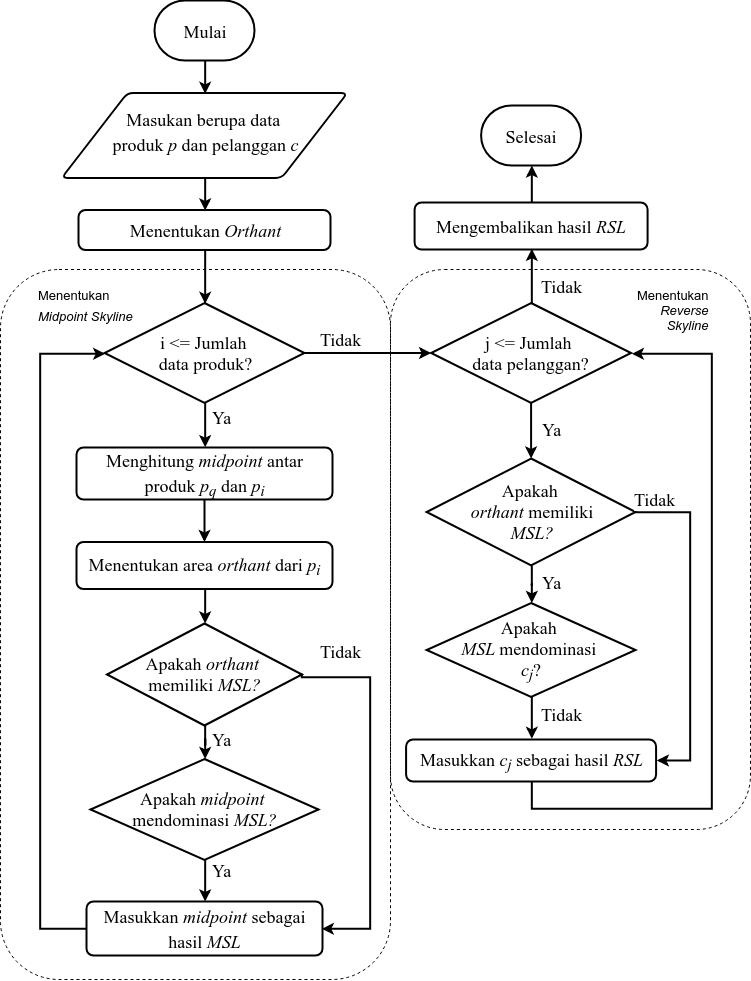
\includegraphics[width=11.5cm]{assets/img/bab3/flowchart-rsl.png}
	\caption{Diagram alir komputasi \textit{reverse skyline}}
	\label{fig:flowchart-rsl}
\end{figure}

\begin{figure}[H]
	\centering
	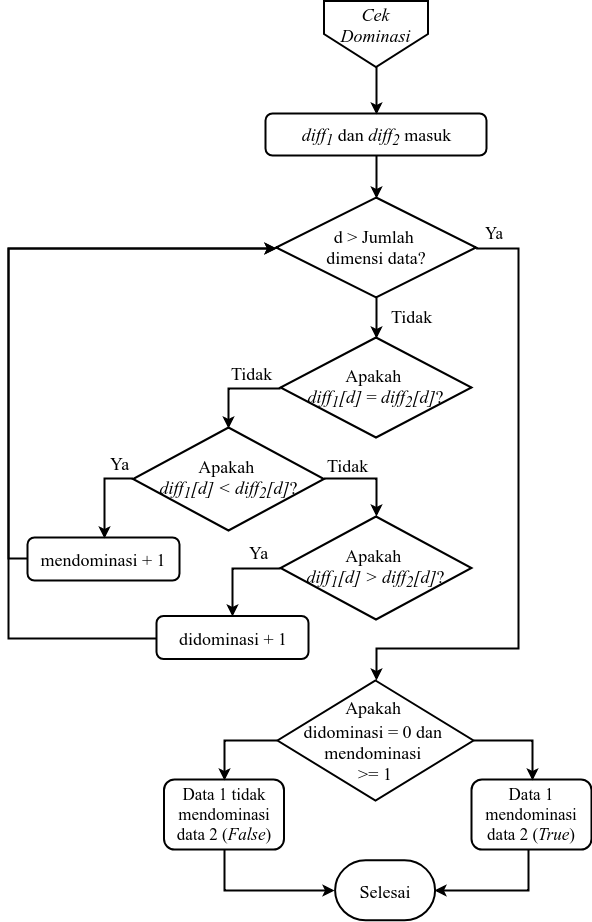
\includegraphics[width=10cm]{assets/img/bab3/flowchart-cek-dom.png}
	\caption{Diagram alir pengecekan dominasi}
	\label{fig:flowchart-cek-dom}
\end{figure}

\subsubsection{\textit{Query Processing}}
\tab \textit{Query processing} adalah algoritme pencarian $k$ produk yang paling menjanjikan dalam interval waktu tertentu. Kueri ini disebut dengan k-MPPTI (\textit{k-Most Promising Products in Time Interval}) yang dinotasikan oleh Persamaan \ref{eq:kmppti}. 
\begin{equation}\label{eq:kmppti}
k-MPPTI(k, [t_i:t_e])
\end{equation} 

Kueri k-MPPTI hanya membutuhkan dua masukan saja, yaitu bilangan bulat positif $k$ yang lebih kecil dari $|P|$ sebagai jumlah produk yang dicari dan interval waktu pencarian yang terdiri dari waktu awal dan waktu akhir $[t_i:t_e]$. Berbeda dengan kueri k-MPP (Persamaan \ref{eq:kmpp}), kueri k-MPPTI tidak membutuhkan masukan \textit{dataset} produk $P$ dan preferensi pelanggan $C$ lagi karena sudah melalui tahap \textit{data precomputing} yang menghasilkan \textit{Pandora Box}.

\begin{figure}[h]
	\centering
	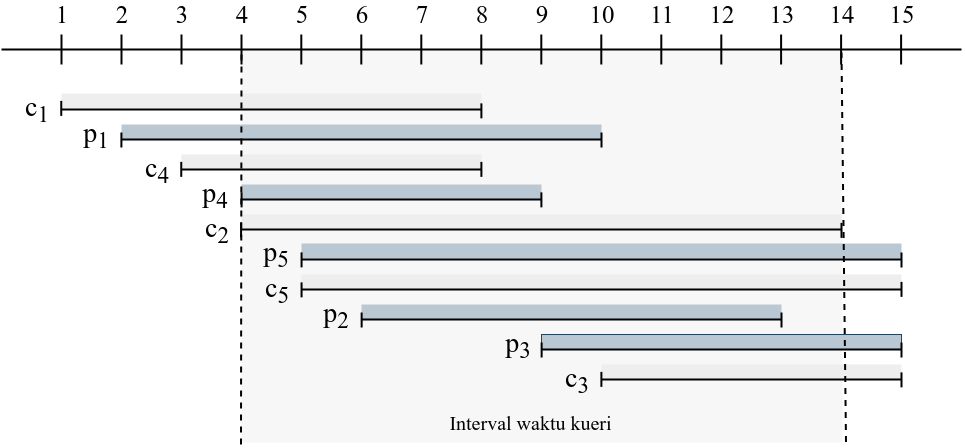
\includegraphics[width=10cm]{assets/img/bab3/timeline-interval.png}
	\caption{Ilustrasi interval waktu pencarian}
	\label{fig:timeline-kueri}
\end{figure}

Algoritme \textit{query processing} mengadaptasi strategi pemilihan produk k-MPP, yakni memilih \textit{subset} $k$ produk $P'$ dari $P$ yang memiliki kontribusi pasar lebih besar dibandingkan dengan \textit{subset} $k$ produk $P''$ dari $P$ yang lain \cite{kmpp} dengan menambahkan interval waktu pencarian. Perhitungan kontribusi pasar dinotasikan dengan Persamaan \ref{eq:market-contr-ti-1} dan \ref{eq:market-contr-ti-2}.
\begin{equation}\label{eq:market-contr-ti-2}
E_{[t_i:t_e]}(CA, p|PA) = \sum_{t=t_i}^{t_e} \sum_{\forall c \in CA} E_t(CA, p|PA)
\end{equation} 
\begin{equation}\label{eq:market-contr-ti-1}
E_{[t_i:t_e]}(CA, p|PA) = \sum_{t=t_i}^{t_e} \sum_{\forall c \in RSL(p)} E_t(CA, p|PA)
\end{equation} 

Ada dua langkah pemrosesan yang harus dilakukan, yaitu (1) mengakumulasi skor kontribusi pasar setiap produk $p \in P$ dalam interval waktu pencarian dan (2) mengurutkan total skor dari yang terbesar dan mengembalikan $k$-produk teratas sebagai hasil dari kueri pencarian. 

\begin{figure}[h]
	\centering
	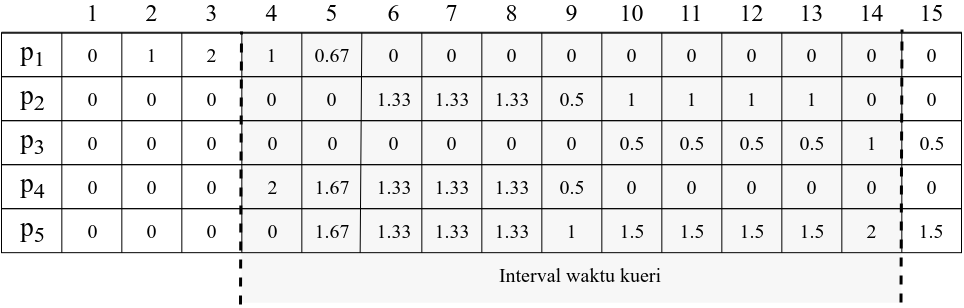
\includegraphics[width=10cm]{assets/img/bab3/pbox-kueri.png}
	\caption{Perhitungan kontribusi pasar pada \textit{Pandora Box} berdasarkan interval waktu pencarian}
	\label{fig:pbox-kueri}
\end{figure}

Misalnya, seorang pengguna ingin mencari $3$ produk yang paling menjanjikan dalam interval waktu $4$ hingga $14$, dinotasikan dengan $k-MPPTI(3, [4:14])$. Berdasarkan hasil perhitungan total kontribusi pasar berbasis interval waktu pada Tabel \ref{tab:mc-ti-res}, produk $p_5$, $p_2$ dan $p_4$ adalah $3$ produk paling menjanjikan dalam interval waktu $4$ hingga $14$.

\begin{table}[H]
	\small
	\centering
	\begin{tabular}{|p{4cm}|p{2cm}|}
		\hline
		$E_{[4:14]}(CA, p_5|PA)$ & $14.67$ \\ \hline
		$E_{[4:14]}(CA, p_2|PA)$ & $8.5$ \\ \hline
		$E_{[4:14]}(CA, p_4|PA)$ & $8.17$ \\ \hline
		$E_{[4:14]}(CA, p_3|PA)$ & $3$ \\ \hline
		$E_{[4:14]}(CA, p_1|PA)$ & $1.67$ \\ \hline
	\end{tabular} 
	\caption{Kontribusi pasar (1)}
	\label{tab:mc-ti-res}
\end{table}

Interval waktu pencarian sangat mempengaruhi hasil kueri. Sebagai bukti, jika interval waktu pencariannya diubah menjadi $1$ hingga $6$, $[1:6]$, maka hasil kueri $3$ produk teratas yang paling menjanjikan adalah $p_4$, $p_1$, dan $p_5$.

\begin{table}[H]
	\small
	\centering
	\begin{tabular}{|p{3cm}|p{2cm}|}
		\hline
		$E_{[4:14]}(CA, p_4|PA)$ & $5$ \\ \hline
		$E_{[4:14]}(CA, p_1|PA)$ & $1.67$ \\ \hline
		$E_{[4:14]}(CA, p_5|PA)$ & $3$ \\ \hline
		$E_{[4:14]}(CA, p_2|PA)$ & $1.33$ \\ \hline
		$E_{[4:14]}(CA, p_3|PA)$ & $0$ \\ \hline
	\end{tabular} 
	\caption{Kontribusi pasar (2)}
	\label{tab:mc-ti-res2}
\end{table}

\subsection{Algoritme Tandingan}
\tab Dalam Tugas Akhir ini juga dibuat algoritme tandingan untuk membandingkan performa algoritme yang dibuat. Ada dua jenis algoritme yang dibuat: (1) algoritme k-MPPTI NoRSL, yaitu algoritme k-MPPTI yang tidak melalui proses komputasi \textit{reverse skyline} dan (2) algoritme k-MPPTI NoRSL-P, yaitu algoritme k-MPPTI NoRSL yang mengimplementasikan teknik pemrosesan paralel.

Teknik pemrosesan paralel, yaitu suatu bentuk komputasi dua atau lebih tugas yang dilakukan secara bersamaan dan beroperasi dengan prinsip bahwa masalah besar seringkali dapat dibagi dan dipecah menjadi masalah yang lebih kecil, kemudian dipecahkan secara bersamaan (paralel) \cite{paralel}. 

\begin{figure}[h]
	\centering
	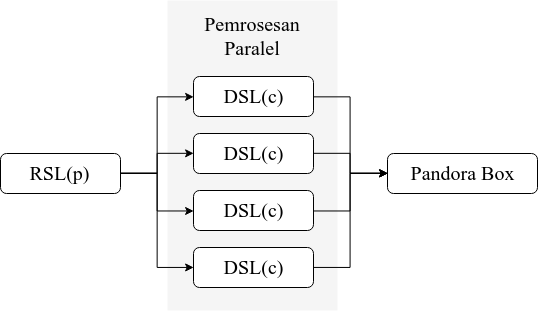
\includegraphics[width=8cm]{assets/img/bab3/paralel.png}
	\caption{Pemrosesan paralel}
	\label{fig:paralel}
\end{figure}

Pemrosesan paralel dilakukan dengan cara menggunakan satu atau lebih CPU atau prosesor untuk menjalankan program atau multi-\textit{thread}. Karena dilakukan secara bersamaan, maka pemrosesan ini hanya dapat dilakukan jika suatu tugas tidak membutuhkan masukan dari keluaran tugas sebelumnya, misalnya komputasi $DSL(c)$ untuk setiap $c \in RSL(p)$ yang diilustrasikan pada Gambar \ref{fig:paralel}.

\subsection{Arsitektur Aplikasi} 
\tab Sistem akan diimplementasikan menggunakan arsitektur \textit{client}-\textit{server} seperti yang diilustrasikan pada Gambar \ref{fig:arsitektur}. Terdapat dua komponen utama dalam arsitektur ini, yaitu klien (\textit{client}), pihak yang meminta atau menerima layanan, dan peladen (\textit{server}), pihak yang memberikan atau mengirim layanan. Komponen-komponen ini terhubung ke jaringan, baik melalui kabel maupun nirkabel untuk melakukan transmisi data. 

\begin{figure}[h]
	\centering
	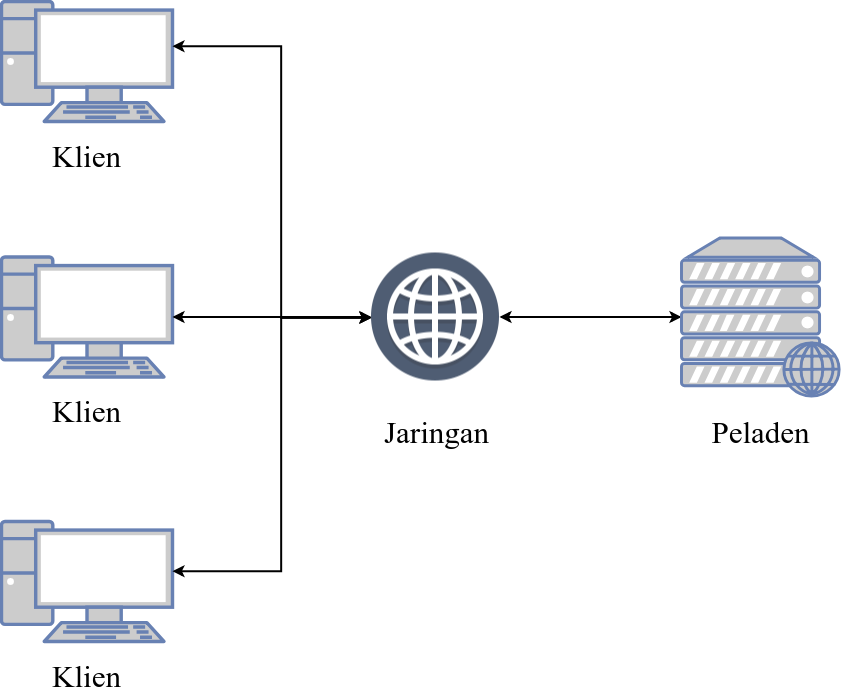
\includegraphics[width=7cm]{assets/img/bab3/arsitektur.png}
	\caption{Perancangan arsitektur aplikasi}
	\label{fig:arsitektur}
\end{figure}

Klien mengimplementasikan antarmuka pengguna grafis atau APG (Inggris: \textit{graphical user interface} atau GUI) berbasis web, sedangkan peladen mengimplementasikan \textit{back-end service} yang berisi algoritme komputasi k-MPPTI yang terdiri atas algoritme \textit{data precomputing} dan \textit{query processing}. Web dibangun menggunakan Flask \textit{microframework} dan bahasa Python, HTML, CSS, serta Javascript, sedangkan \textit{back-end service} diimplementasikan menggunakan bahasa Python. Flask juga sekaligus berperan sebagai peladen web (\textit{web server}).

Pengguna melakukan masukan data melalui web, kemudian data tersebut dikirimkan ke \textit{back-end service} untuk dilakukan proses \textit{data precomputing}. Setelah hasil \textit{data precomputing} selesai, pengguna melakukan masukan kueri pencarian. Kueri pencarian tersebut akan dikirimkan ke \textit{back-end service} untuk dilakukan proses \textit{query processing}. Hasil yang didapatkan akan dikembalikan ke klien, disertai dengan visualisasi data menggunakan pustaka Vis.js.
